\documentclass[12pt]{article}

\usepackage{amsmath}
\usepackage{amssymb}
\usepackage{fancyhdr}
\usepackage{todonotes}
\usepackage{amsthm}
\usepackage{amsopn}
\usepackage{amsfonts}
\usepackage{mathtools}
\usepackage{libertine}

\newtheorem*{theorem}{Theorem}
\newtheorem*{definition}{Definition}
\newtheorem*{remark}{Remark}
\newtheorem*{claim}{Claim}
\newtheorem*{example}{Example}
\newtheorem*{prop}{Proposition}
\newtheorem*{sol}{Solution}

\usepackage{latexsym}
\usepackage{bbm}
\usepackage[small,bf]{caption2}
\usepackage{graphics}
\usepackage{epsfig}
\usepackage{amsopn}
\usepackage{url}

\usepackage[parfill]{parskip}
\usepackage[margin=1in]{geometry}

\newcommand{\bc}{\binom}
\newcommand{\bx}{\boxed}
\newcommand{\RR}{\mathbb{R}}
\newcommand{\CC}{\mathbb{C}}
\newcommand{\DD}{\mathbb{D}}
\newcommand{\QQ}{\mathbb{Q}}
\newcommand{\II}{\mathbb{I}}
\newcommand{\Ra}{\mathcal{R}}
\newcommand{\EE}{\mathbb{E}}
\newcommand{\HH}{\mathcal{H}}
\newcommand{\NN}{\mathbb{N}}
\newcommand{\FF}{\mathbb{F}}
\newcommand{\ve}{\varepsilon}
\newcommand{\eps}{\epsilon}
\newcommand{\la}{\langle}
\newcommand{\ra}{\rangle}
\newcommand{\mbf}{\mathbf}
\newcommand{\ds}{\displaystyle}
\newcommand{\ol}{\overline}

% From stackexchange
\DeclarePairedDelimiterX\set[1]\lbrace\rbrace{\def\given{\;\delimsize\vert\;}#1}
\DeclarePairedDelimiter\abs{\left \lvert}{\right \rvert}%

\DeclareMathOperator{\sign}{sign}
\DeclareMathOperator{\res}{res}
\DeclareMathOperator{\Aut}{Aut}
\DeclareMathOperator{\GL}{GL}
\DeclareMathOperator{\Ker}{Ker}
\DeclareMathOperator{\im}{im}
\DeclareMathOperator{\Syl}{Syl}
%\newcommand{\mat}[4]{\begin{pmatrix} #1 & #2 \\ #3 & #4\end{pmatrix}}
\newcommand*{\mat}[1]{\begin{pmatrix}#1\end{pmatrix}}


\usepackage[parfill]{parskips
\usepackage[margin=1in]{geometry}

\pagestyle{fancy}

\newcommand{\UU}{\mathcal{U}}
\newcommand{\T}{\text}

\newcommand{\eq}[1]{\begin{align*}#1\end{align*}}

\def\Ber{\text{Ber}}
\def\ub{\underbrace}
\def\UU{\mathcal{U}}
\def\WW{\mathcal{W}}
\def\XX{\mathcal{X}}
\def\VV{\mathcal{V}}
\def\Unif{\text{Unif}}
\def\Xh{\hat{X}}
\def\P{\text{P}}
\def\PP{\mathbb{P}}
\def\CC{\mathbb{C}}
\def\KK{\mathbb{K}}
\def\ZZ{\mathbb{Z}}
\def\lb{\lambda}
\def\rot{\text{rot}}

\title{MATH 116 - Complex Analysis}
\author{Instructor: Yakov Eliashberg; Notes: Adithya Ganesh}

\lhead{MATH 116}

\newcommand*{\mat}[1]{\begin{pmatrix}#1\end{pmatrix}}
\begin{document}
\maketitle

\tableofcontents

\section{9-24-18: Introduction}
We can build up complex numbers with a few basic axioms.

\begin{enumerate}
  \item $(1, 0)$ - unit.
  \item $(0, 1)^2 = - (1, 0)$.
  \item Bi-linear in $z_1, z_2$ (i.e. linear with respect to each argument).
\end{enumerate}

Suppose $z = x+iy$.  We define the {\it conjugation} operator as $\ol{z} = x - iy$, such that
\[
  z \ol{z} = x^2 + y^2 = |z|^2.
\]
We can also express $z$ in polar coordinates, so that
\[
  z = x + iy = r(\cos \phi + i \sin \phi).
\]

We can extend the Taylor series of the exponential function on the real line to the complex plane by defining:
\[
  e^z = 1 + z + \frac{z^2}{2!} + \dots + \frac{z^n}{n!} + \dots.
\]
It is easy to check that this definition satisfies the usual properties:
\[
  e^{z_1 + z_2} = e^{z_1} \cdot e^{z_2}; \qquad e^{x + iy} = e^x e^{iy}.
\]
  We can similarly define
  \[
    \cos z = 1 - \frac{z^2}{2} + \frac{z^4}{4!} + \dots.
  \]
  \[
    \sin z = z - \frac{z^3}{3!} + \frac{z^5}{5!} + \dots.
  \]
  We can combine these formulae to obtain $e^{iy} = \cos y + i \sin y$ (Euler).

  Combining this with the previous definition, we can write
  \[
    r e^{i \phi} = r (\cos \phi + i \sin \phi).
  \]

  Now, if $z = re^{i \phi}$, we can write $z^{-1} = \frac{1}{r} e^{-i \phi}$.  This gives you a very natural geometric interpretation of inversion (conjugation + scaling).

  Note that it is straightforward to derive trigonometric identities from Euler's formula; for example it is easy to see that
  \[
    (\cos \phi + i \sin \phi)^n = \cos n \phi + i \sin n \phi.
  \]

  {\it Linear functions.}  Suppose we have a linear map $F: \RR^2 \to \RR^2$.  We can write this as
  \[
    F \mat{x \\ y} = \mat{a & b \\ c & d} \mat{x \\ y}.
  \]
  And furthermore, the following axioms must be satisfied:
  \begin{itemize}
    \item $F(z_1 + z_2) = F(z_1) + F(z_2)$.
    \item $F(\lambda z) = \lambda F(z)$.
  \end{itemize}

  One question: we could have either $\lambda \in \RR$ (termed a real linear map) or $\lambda \in \CC$ (termed a complex valued linear map).

  If $F$ is a complex linear map, we must have $F(iz) = i F(z)$ (i.e. the matrix has to commute).  Furthermore, we must have $F(z) = F(z \cdot 1) = z F(1) = c$, where $c = a+ib$.  So
  \[
    F(z) = (a+ib) (x+iy) = (ax - by) + (ay + bx)i.
    \]
    Also,
    \[
      \mat{a & -b \\ b & a} \mat{x \\ y} = \mat{ax - by \\ ay + bx}.
      \]
      It follows that $F$ is complex if and only if $a = d$ and $b = -c$.


      If $z = x+iy$, we can write $x = \frac{1}{2} (z + \ol{z})$ and $y = - \frac{i}{2} (z - \ol{z})$.  Now, set $A = a+ic$, $B = b + id$, so we can write.

      \[
        \frac{1}{2} (A - iB) z  \frac{1}{2} (A + iB) \ol{z} = \alpha z + \beta \ol{z}.
      \]
      Importantly, $\alpha z$ is complex linear while $\beta \ol{z}$ is complex antilinear (which means $F(\lambda z) = \ol{\lambda} F(z)$.

        This proves that any real linear map can be written as a sum of a complex linear map and a complex antilinear map.

        \newpage

        \section{Differential 1-forms}

        Here, $\RR^2_z$ denotes the space $\RR^2$ with the origin shifted to the point $z$.  A differential 1-form is a function of arguments of 2 kinds: of a point $z \in U$ and a vector $h \in \RR_z^2$.  It depends linearly on $h$ and arbitrarily (but usually continuously and even differentiably) on $z$.

        We will need only 1-forms on domains in $\RR^2$.  A differential 1-form $\lambda$ on a domain $U \subset \RR^2$ is a field of linear functions $\lambda_{z} = \RR_z^2 \to \RR$.  Thus a 1-form is a function of arguments of 2 kinds: of a point $z \in U$ and a vector $h \in \RR_z^2$.  

        Given a real valued function $f: U \to \RR^2$ on $U$, its differential $df$ is an example of a differential form: $d_z(f)(h) = \frac{\partial f}{\partial x} h_1 + \frac{\partial f}{\partial y} h_2$.  In particular, differentials $dx$ and $dy$ of the coordinate functions $x, y$ are differential 1-forms.  Any other differential form can be written as a linear combination of $dx$ and $dy$:
        \begin{align*}
          \lambda = P dx +  Q dy,
        \end{align*}
        where $P, Q: U \to \RR$ are functions on the domain $U$.

        A differential 1-form $\lambda$ is exact if $\lambda = df$.  The function $f$ is called the primitive of the 1-form $\lambda$.  The necessary condition for exactness if that $\lambda$ is closed which by definition means $\frac{\partial P}{\partial y} = \frac{\partial Q}{\partial x}$.

        \section{Complex projective line, or Riemann sphere}

        Consider the space $\CC^n$.  Similar to the real case, one can {\it projectivise} $\CC^n$.  $\CC P^n$ is defined as the space of all complex lines through the origin.  For us, the one-dimensional complex projective space is most relevant, the complex projective line ($\CC P^1$).

        Any vector $z = (z_1, z_2) \in \CC^2$ generates the 1-dimensional complex subspace (complex line) denoted as
        \begin{align*}
          l_z = \Span(z) = \left\{ \lambda z: \lambda \in \CC \right\}.
        \end{align*}

        This line $l_z$ can be viewed as a point of $\CC P^1$.  Any proportional vector $\ol{z} = \mu z$ generates the same line.  Fix an affine line $L_1 = \left\{ z_2 = 1 \right\} \subset \CC^2$.  Any line from $\CC P^1$ except $\left\{ z_2 = 0 \right\}




        \section{Riemann surfaces}


        A Riemann surface is a 1-dimensional complex manifold.  A set $S$ is called a Riemann surface if there exist subsets $U_{\lambda} \subset X, \lambda \in \Delta$, where $\Delta$ is a finite of countable set of indices, and for every $\lambda \in \Delta$ a map $\Phi_{\lambda}: U_{\lambda} \to \C$ such that

        \begin{itemize}
          \item $S = \bigcup_{\lambda \in \Delta}$
          \item The image $G_{\lambda} = \Phi_{\lambda} (U_{\lambda})$ is an open set in $\CC$.
          \item The map $\Phi_{\lambda}$ viewed as a map $U_{\lambda} \to G_{\lambda}$ is one to one.
          \item For any two sets $U_{\lambda}, U_{\mu}, \lambda, \mu \in \Delta$, the images $\Phi_{\lambda} (U_{\lambda} \cap U_{\mu}), \Psi_{\mu} (U_{\lambda} \cap U_{\mu}) \subset \C$ are open and the map
            \begin{align*}
              h_{\lambda, \mu} = \Phi_{\mu} \circ \Phi_{\lambda}^{-1} : \Phi_{\lambda} (U_{\lambda} \cap U_{\mu}) \to \Phi_{\mu} (U_{\lambda} \cap U_{\mu}) \subset \R^n
            \end{align*}
        \end{itemize}



        \section{Key ideas}

        \subsection{Basic facts}

        \begin{enumerate}
          \item $e^z = \sum_{n=0}^{\infty} \frac{z^n}{n!}$.
          \item $\sin z = \sum_{n=0}^{\infty} (-1)^{n} \frac{z^{2n+1}}{(2n+1)!}$
          \item $\cos z = \sum_{n=0}^{\infty} (-1)^{n} \frac{z^{2n}}{(2n)!}$.
        \end{enumerate}

        \subsection{Main results} 

        {\bf Cauchy's integral formulas.}

        Suppose $f$ is holomorphic on an open set that contains the closure of a disc $D$.  If $C$ denotes the boundary circle of this disc with the positive orientation, then
        \begin{align*}
          f(z) = \frac{1}{2 \pi i} \int_{C} \frac{f(\zeta)}{z - \zeta} \, d \zeta.
        \end{align*}

        {\bf Cauchy's integral formulas for derivatives.}

        Let $f$ be holomorphic on an open set $\Omega$, then $f$ has infinitely many complex derivatives in $\Omega$.  Moreover, if $C \subset \Omega$ is a circle whose interior is also contained in $\Omega$, then
        \begin{align*}
          f^{(n)} (z) = \frac{n!}{2 \pi i} \int_{C} \frac{f(\zeta)}{(\zeta - z)^{n+1}} \, d \zeta.
        \end{align*}

        {\bf Cauchy-Riemann.} $f$ is analytic iff $u_x = v_y$, $u_y = - v_x$.

        {\bf $C^1$ class.} Every holomorphic function is a domain $U$ is of class $C^1$, i.e. its derivative continuously depends on the point of $U$.

        {\bf Cauchy's theorem.}

        {\bf Liouville's theorem.} If $f$ is entire and bounded, then $f$ is constant.

        {\bf Singularities and poles.} A point singularity (or isolated singularities) of $f$ is a $z_0 \in \CC$ such that $f$ is defined in a neighborhood of $z_0$ but not at the point $z_0$ itself.  A zero for the holomorphic function $f$ is $z_0$ such that $f(z_0) = 0$.  By analtic continuation, the zeros of a non-trivial holomorphic function are isolated.  A function $F$ defined in a deleted neighborhood of $z_0$ has a pole at $z_0$ if the function $\frac{1}{f}$, defined to be to be zero at $z_0$, is holomorphic in a full neighborhood of $z_0$.

        {\bf Pole power series representation.}  If $f$ has a pole of order $n$ at $z_0$, then
        \begin{align*}
          f(z) = \frac{a_{-n}}{(z-z_0)^n} + \frac{a_{-n+1}}{(z - z_0)^{n-1}} + \cdots + \frac{a_{-1}}{(z - z_0)} + G(z),
        \end{align*}
        where $G$ is a holomorphic function in a neighborhood of $z_0$.

        {\bf Residue at a pole.}  The residue of $f$ at that pole is defined as the coefficient $a_{-1}$, so that $\res_{z_0} f = a_{-1}$.  In particular, if $f$ has a pole of order $n$ at $z_0$, then
        \begin{align*}
          \res_{z_0} f = \lim_{z \to z_0} \frac{1}{(n-1)!} \left( \frac{d}{dz} \right)^{n-1} (z - z_0)^n f(z).
        \end{align*}

        {\bf Residue formula, and corollary.} Suppose that $f$ is holomorphic in an open set containing a circle $C$ and its interior, except for a pole at $z_0$ inside $C$.  Then
        \begin{align*}
          \int_{C} f(z) \, dz = 2 \pi i \res_{z_0} f.
        \end{align*}

        Suppose $f$ is holomorphic on an open set containing a circle $C$ and its interior, except for poles at the points $z_1, \cdots, z_N$ inside $C$.  Then

        \begin{align*}
          \int_{C} f(z) \, dz = 2 \pi i \sum_{k=1}^{N} \res_{z_k} f.
        \end{align*}
 
        {\bf Conformal map.} A bijective holomorphic function $f: U \to V$ is called a conformal map or biholomorphism.

        {\bf Riemann mapping theorem.} Suppose $\Omega$ is proper and simply connected.  If $z_0 \in \Omega$, then there exists a unique conformal map $F: \Omega \to \DD$ such that 
        \[
          F(z_0) = 0; \qquad F'(z_0) > 0.
        \]

        {\bf Corollary (3.2)} Any two proper simply connected open subsets in $\CC$ are conformally equivalent.

        {\bf Mantel's theorem.}


        \newpage
        \section{Midterm review sheet}

        \subsection{Cauchy-Riemann equations}

        $f$ is holomorphic iff $u_x = v_y; u_y = - v_x$.

        Differential operators w.r.t. $z$ and $\ol{z}$.

        \begin{align*}
          \frac{\partial}{\partial z} &= \frac{1}{2} \left( \frac{\partial}{\partial x} + \frac{1}{i} \frac{\partial }{\partial y} \right) \\
          \frac{\partial}{\partial \ol{z}} &= \frac{1}{2} \left( \frac{\partial}{\partial x} - \frac{1}{i} \frac{\partial }{\partial y} \right).
        \end{align*}

        \subsection{Cauchy integral formula + applications}

        Suppose $f$ is holomorphic on an open set that contains the closure of a disc $D$.  If $C$ is the boundary circle, then for any $z \in D$:
        \begin{align*}
          f(z) = \frac{1}{2 \pi i} \int_{C} \frac{f(\zeta)}{\zeta - z} \, d \zeta.
        \end{align*}

        {\it $n$-th derivative.} If $f$ is holomorphic in an open se T$\Omega$, then $f$ has infinitely many complex derivatives in $\Omega$.  If $C \subset \Omega$ is a cricle whose interior is only contained in $\Omega$, then for all $z$ in the interior of $C$:
        \[
          f^{(n)}(z) = \frac{n!}{2\pi i} \int_{C} \frac{f(\zeta)}{(\zeta - z)^{n+1}} d \, zeta.
        \]

        {\it Cauchy inequality + quick proof.} If $f$ is holomorphic in an open set that contains the closure of a disc $D$ centered at $z_0$ and of radius $R$, then
        \[
          |f^{(n)}(z_0)| \leq \frac{n! ||f||_C}{R^n}.
        \]

        \begin{proof}
          By the Cauchy integral formula, we obtain
          \begin{align*}
            |f^{(n)}(z_0)| &= \left | \frac{n!}{2 \pi i} \int_{C} \frac{f(\zeta)}{(\zeta - z_0)^{n+1}} \, d \zeta \right | \\
            &= \frac{n!}{2 \pi} \left | \int_{0}^{2 \pi} \frac{f(z_0 + Re^{i \theta})}{(Re^{i \theta})^{n+1}} Ri e^{i \theta} d \theta \right | \\
            & \leq \frac{n!}{2 \pi} \frac{||f||_C}{R^n} 2\pi.
          \end{align*}
        \end{proof}

        {\bf Liouville's theorem.} If $f$ is entire and bounded, then $f$ is constant.

        \begin{proof}
          By Cauchy inequality, we obtain
          \begin{align*}
            |f'(z_0)| \leq \frac{B}{R},
          \end{align*}
          where $B$ is some bound for $f$.  Taking $R \to \infty$, we obtain the desired result.
        \end{proof}

        {\bf Quick proof of FTA.} Suppose $P$ has no roots.  Then $\frac{1}{P(z)}$ is bounded and entire.  But then $\frac{1}{P(z)}$ is constant, which is a contradiction.

        {\bf Schwarz reflection principle.} Suppose that $f$ is a holomorphic function in $\Omega^{+}$ that extends continuously to $I$ and such that $f$ is real-valued on $I$.  Then there exists a function $F$ holomorphic in all of $\Omega$ such that $F = f$ on $\Omega^{+}$.

        \begin{proof}
          For $z \in \Omega^{-}$, define $F(z)$ by
          \[
            F(z) = \ol{f(\ol{z})},
          \]
          look at power series expansions, and invoke the symmetry principle.
        \end{proof}

        \subsection{Power series}

        Suppose $f$ is holomorphic in an open set $\Omega$.  If $D$ is a disc centered at $z_0$ and whose closure is contained in $\Omega$, then $f$ has a power series expansion at $z_0:$
        \[
          f(Z) = \sum_{n=0}^{\infty} a_n (z- z_0)^n,
        \]
        where $a_n = \frac{f^{(n)}(z_0)}{n!}$.


        {\bf Analytic continuation.}  Suppose $f$ and $F$ are analytic in regions $\Omega, \Omega'$ with $\Omega \subset \Omega'$.  If the two functions agree on the smaller set $\Omega$, then $F$ is an analytic continuation of $f$ into the region $\Omega'$, and is uniquely determined by $f$.

        In particular, suppose $f$ and $g$ are holomorphic in a region $\Omega$ and $f(z) = g(z)$ for all $z$ in some non-empty open subset of $\Omega$.  Then $f(z) = g(z)$ throughout $\Omega$.

        \subsection{Exponential function and logarithm}

        {\bf Complex logarithm.} Write
        \[
          \log z = \log r + i \theta;
        \]
        principal branch when $|\theta| < \pi$.  Constructively, we can write
        \[
          \log_{\Omega}(z) = F(z) = \int_{\gamma} f(w) \, dw,
        \]
        where $\gamma$ is any curve connecting $1$ to $z$.  Standard path of integration is to take $1 \to r \in \RR$ and then $r \to z$, so that
        \begin{align*}
          \log z &= \int_{1}^{r} \frac{dx}{x} + \int_{\eta} \frac{dw}{w} \\
          &= \log r + \int_{0}^{\theta} \frac{i r e^{it}}{r e^{it}} \, dt \\
          &= \log r + i \theta.
        \end{align*}

        Note that in general
        \[
          \log(z_1 z_2) \neq \log z_1 + \log z_2.
        \]

        {\bf Taylor expansion for $\log(1+x)$.} For the principal branch, we can write
        \[
          \log(1+z) = z - \frac{z^2}{2} + \frac{z^3}{3} - \dots.
        \]




        \subsection{Meromorphic functions}

        {\bf Definition of a meromorphic function.} A function $f$ on an open set $\Omega$ is meromorphic if there exists a sequence of points $z_0, z_1, \dots$ that has no limit points in $\Omega$ and such that

        \begin{itemize}
          \item $f$ is holomorphic in $\Omega \setminus \left\{ z_0, z_1, \dots \right\}$
          \item $f$ has poles at the points $\left\{ z_0, z_1, \dots \right\}$.
        \end{itemize}

        {\bf Casorati-Weierstrass.} Suppose $f$ is holomorphic in the punctured disc $D_r(z_0) \setminus \left\{ z_0 \right\}$ and has an essential singularity  at $z_0$.  Then the image of $D_r(z_0) - \left\{ z_0 \right\}$ under $f$ is dense in the complex plane.

        \subsection{Argument principle and Rouche's theorem}

        {\bf Argument principle.} Suppose $f$ is meromorphic in an open set containing a circle $C$ and its interior.  If $f$ has no poles and never vanishes on $C$, then

        \[
          \frac{1}{2 \pi i} \int_{C} \frac{f'(z)}{f(z)} \, dz =Z - P,
        \]
        where $Z$ is the number of zeros inside $C$, and $P$ is the number of poles inside $C$.

        {\bf Rouche's theorem.} Suppose that $f$ and $g$ are holomorphic in an open set containing a circle $C$ and its interior.  If $|f(z)| < |g(z)|$ for all $z \in C$, then $f$ and $f+g$ have the same number of zeros inside $C$.

        \begin{proof}
          Let $f_t(z) = f(z) + t g(z); t \in [0, 1]$.
          Argue that
          \[
            n_t = \frac{1}{2 \pi i} \int_{C} \frac{f_t'(z)}{f_t(z)} \, dz
            \]
            is constant; and in particular that $n_0 = n_1$.
        \end{proof}

        {\bf Open mapping theorem.} If $f$ and holomorphic and nonconstant in a region $\Omega$, then $f$ is open.

        {\bf Maximum modulus principle.} If $f$ is a nonconstant holomorphic function in a region $\Omega$, then $f$ cannot attain a maximum in $\Omega$.

        \begin{proof}
          Immediate from open mapping theorem.
        \end{proof}

        \subsection{Computation of integrals using residues}

        {\bf Residue limit identity.} If $f$  has a pole of order $n$ at $z_0$, then
        \[
          \res_{z_0} f = \lim_{z \to z_0} \frac{1}{(n-1)!} \left( \frac{d}{dz} \right)^{n-1} (z - z_0)^n f(z).
        \]

        {\bf Residue theorem.} Suppose that $f$ is holomorphic in an open set containing a toy contour $\gamma$ and its interior, except for poles at the points $z_i$ inside $\gamma$.  Then
        \[
          \int_{\gamma} f(z) \, dz =2 \pi i \sum_{k=1}^{N} \res_{z_k} f.
          \]

          {\bf Integrals to know.}

          \begin{itemize}
            \item $\int_{- \infty}^{\infty} \frac{dx}{1+x^2} = \pi$.
            \item $\int_{- \infty}^{\infty} \frac{e^{ax}}{1 + e^x}\, dx = \frac{\pi}{ \sin \pi a}; 0 < a < 1$.
            \item $\int_{- \infty}^{\infty} \frac{e^{- 2 \pi i x \xi}}{\cosh \pi x} \, dx = \frac{1}{\cosh \pi \xi}$.
          \end{itemize}
        

        \subsection{Harmonic functions and harmonic conjugates}

        {\bf Definition.} A real of complex valued $C^2$-smooth function $f$ on a domain $U \subset \CC$ is harmonic if
          \[
            \frac{\partial^2 f}{\partial x^2} + \frac{\partial^2 f}{\partial y^2} = 0.
          \]

          {\bf Unique determination.} let $f, g : U \to \RR$ be two harmonic functions which extend continuously to the boundary $\partial U$.  Suppose that $f = g$ on $\partial U$.  Then $f = g$ on $U$.

          \begin{proof}
            Suppose for $a \in U$ we have $f(a) > g(a)$; then consider $f - g$ and apply maximum modulus principle; contradiction.
          \end{proof}

          {\bf Log-composition.} If $f$ is a holomorphic function then $h(z) = \ln |f(z)|$ is harmonic.

          {\bf Harmonic conjugate.} The harmonic conjugate to a function $u(x, y)$ is a function $v(x, y)$ such that $u + iv$ is analytic.

          {\it Example.} The harmonic conjugate of $u(x, y) = e^x \sin y$ is $- e^{x} \cos y + C$.

        \subsection{Elementary conformal mappings}

        Examples to know:

        \begin{center}
          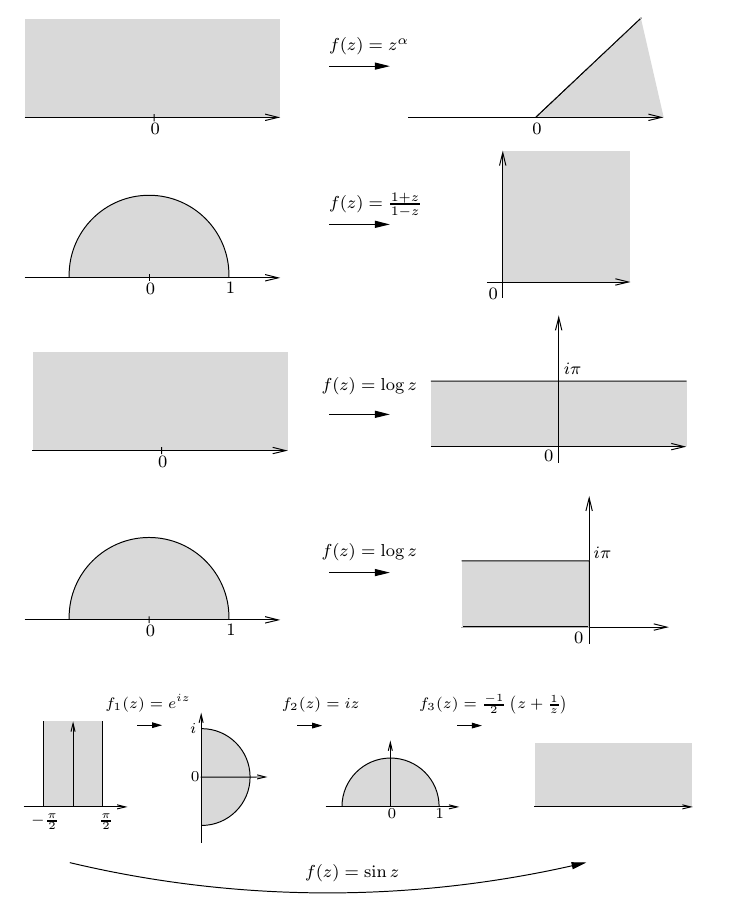
\includegraphics[width=0.6\textwidth]{conformal}
        \end{center}

        \subsection{Properties of fractional linear transformations}

        Fractional linear transformations are mappings of the form
        \[
          z \mapsto \frac{az + b}{cz + d}.
        \]

        They always map circles and lines to circles and lines.

        %\subsection{Compiled problem set}

        % HW1
        %\begin{enumerate}
          %\item 
            %\begin{enumerate}
              %\item Solve the equation $|z| - z = a + bi$.
              %\item Compute $(1 + \cos \alpha + i \sin \alpha)^n$.
              %\item Prove that
                %\begin{align*}
                  %1 + \binom{n}{3} + \binom{n}{6} + \cdots = \frac{1}{3} \left( 2^n + 2 \cos \frac{\pi n}{3} \right).
                %\end{align*}
            %\end{enumerate}
          %\item Let $f: U \to \CC$ be a holomorphic function, where $U$ is a connected domain.  Suppose that $|f(z)| = 1$ for all $z \in U$.  Show that $f(z)$ is constant.
          %\item Prove that a function $f(z)$ is holomorphic in a domain $U$ if and only if the function $\ol{f(\ol{z})}$ is holomorphic in the domain $\ol{U} = \left\{ z \in \CC; \ol{z} \in U \right\}$.
          %\item Write the Cauchy-Riemann equations in polar coordinates.
          %\item Let $f(z) = x^3 - 3xy^2 + i (3x^2 y - y^3)$, $z = x + iy$.  Compute $\frac{\partial f}{\partial z}$ and $\frac{\partial f}{\partial \ol{z}}$.  Is this function holomorphic?
          %\item Compute integrals:
            %\begin{enumerate}
          %\item $\int_{\Gamma} |z| \, dz$, where $\Gamma$ is the interval $[-i, i]$ on the imaginary axis, oriented from $-i$ to $i$.
          %\item $\int_{\Gamma} (6z^5 - 5z^4 + 4z^2 - 1) \, dz$, where $\Gamma$ is given by the parametric equations
            %\begin{align*}
              %x(t) &= \sin^3 t - 2 \cos t + 3 \\
              %y(t) &= \sin^2 2t - \sin^5 4t; \quad t \in [0, \frac{\pi}{2} ]
            %\end{align*}
            %\end{enumerate}
        \end{enumerate}



\end{document}
